% !TEX root = ../1-main-SL.tex
% !TEX encoding = UTF-8  (utf8)

\begin{frame}
	\centering
	\bf\Huge\color{purple} 习题1-2讲评\\[1cm]
	\small\color{gray}2018-10-24
\end{frame}

\section{说在前面}

\begin{frame}[t]\frametitle{说在前面}
	\linespread{1.8}
	\Large
    \begin{itemize}
    	\item 如何改错?
    	\begin{enumerate}
    		\item {\it\Large 多留空白...}
    		\item {\it\Large 要还是不要,划清界限...}
    	\end{enumerate}
    	\item 对还是错?
    	\begin{enumerate}
    		\item {\it\Large $\sqrt[3]{n+1}-\sqrt[3]{n}<\sqrt{n+1}-\sqrt{n}$.}
    		\item {\it\Large 要证$\limn(a_{n+1}-a_n)=0$,只需证明}
    		$$\limn\df{a_{n+1}}{a_n}=1.$$
    		\item {\it\Large $\{a_n\}$有界,故可设$\limn a_n=A$.}
    	\end{enumerate}
    \end{itemize}
\end{frame}

\section{参考解答}

\begin{frame}[t]\frametitle{1.用极限的定义证明}
\large
(1)$\limn\df{\sqrt{n^2+a^2}}n=1$;

证:\it 对任意$\e>0$,令$N=\left[\df{a^2}{\e}\right]+1>\df{a^2}{\e}$,
则对任意$n>N$,均有
$$\left|\df{\sqrt{n^2+a^2}}n-1\right|
=\df{a^2}{n(\sqrt{n^2+a^2}+n)}<\df{a^2}n<\df{a^2}N<\e,
$$
由数列极限的定义,即证。\fin
\end{frame}

\begin{frame}[t]\frametitle{1.用极限的定义证明}
\large

(2)$\limn0.\underbrace{99\ldots9}_{n\mbox{\footnotesize 个}}=1.$

证:\it 对任意$\e>0$,令$N=[-\lg\e]+1$,则对任意$n>N$,均有
$$|0.\underbrace{99\ldots9}_{n\mbox{\footnotesize 个}}-1|
=\df1{10^n}<\df1{10^N}
<\df1{10^{-\lg\e}}=\e,$$
由数列极限的定义,即证。\fin
\end{frame}

\begin{frame}[t]\frametitle{1.用极限的定义证明}
\large

(3)$\limn\left(\sqrt[3]{n+1}-\sqrt[3]{n}\right)=0$.
\bs

证:\it 对任意$\e>0$,令$N=\left[1/\e\right]+1$,则对任意$n>N$,有
$$|\sqrt[3]{n+1}-\sqrt[3]{n}|
=\df1{(n+1)^{\frac{2}{3}}+(n+1)^{\frac13}n^{\frac13}+n^{\frac23}}
<\df1n<\df1N<\e.$$
由数列极限的定义,即证。\fin
\end{frame}

\begin{frame}[t]\frametitle{1.用极限的定义证明}
\large

(4)$\limn\df{n^2-n-1}{2n^2+2n-4}=\df12$.
\bs

证:\it 对任意$\e>0$,令$N=$,则对任意$n>N$有
$$\left|\df{n^2-n-1}{2n^2+2n-4}-\df12\right|
=\left|\df{-2n-3}{2n^2+2n-4}\right|<\df1n<\df1N<\df1{\e}.$$
由数列极限的定义,即证。\fin
\end{frame}

\begin{frame}[t]\frametitle{证明极限的性质}
\large
2.数列$\{a_n\}$有界,$\limn b_n=0$,证明:$\limn a_nb_n=0$。
\end{frame}

\begin{frame}{哪里不太对?}
	\centering
	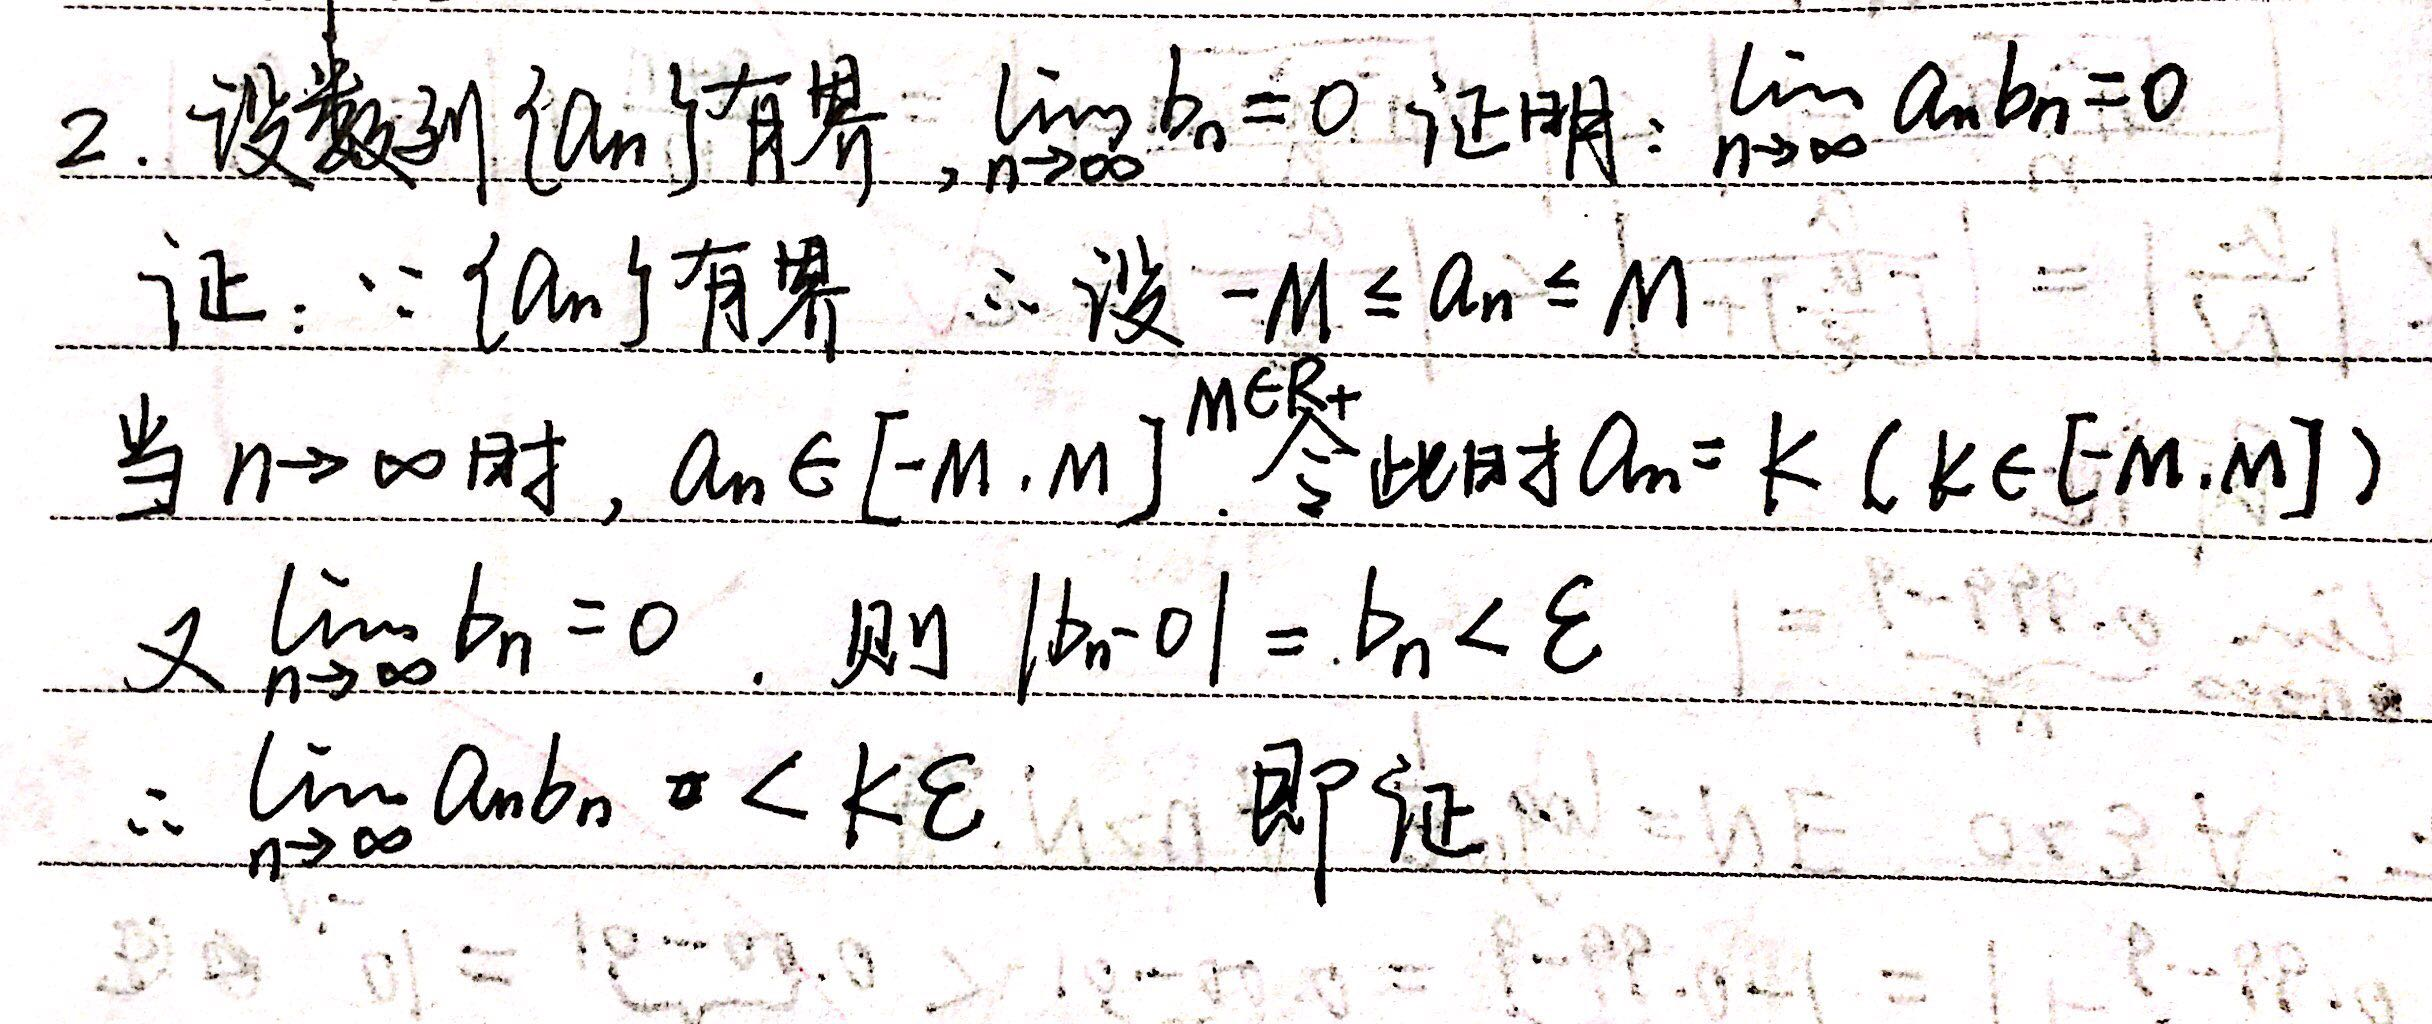
\includegraphics[width=0.9\textwidth]{./images/ch01/HWR/anbn0-1.jpeg}
\end{frame}

\begin{frame}{哪里不太对?}
	\centering
	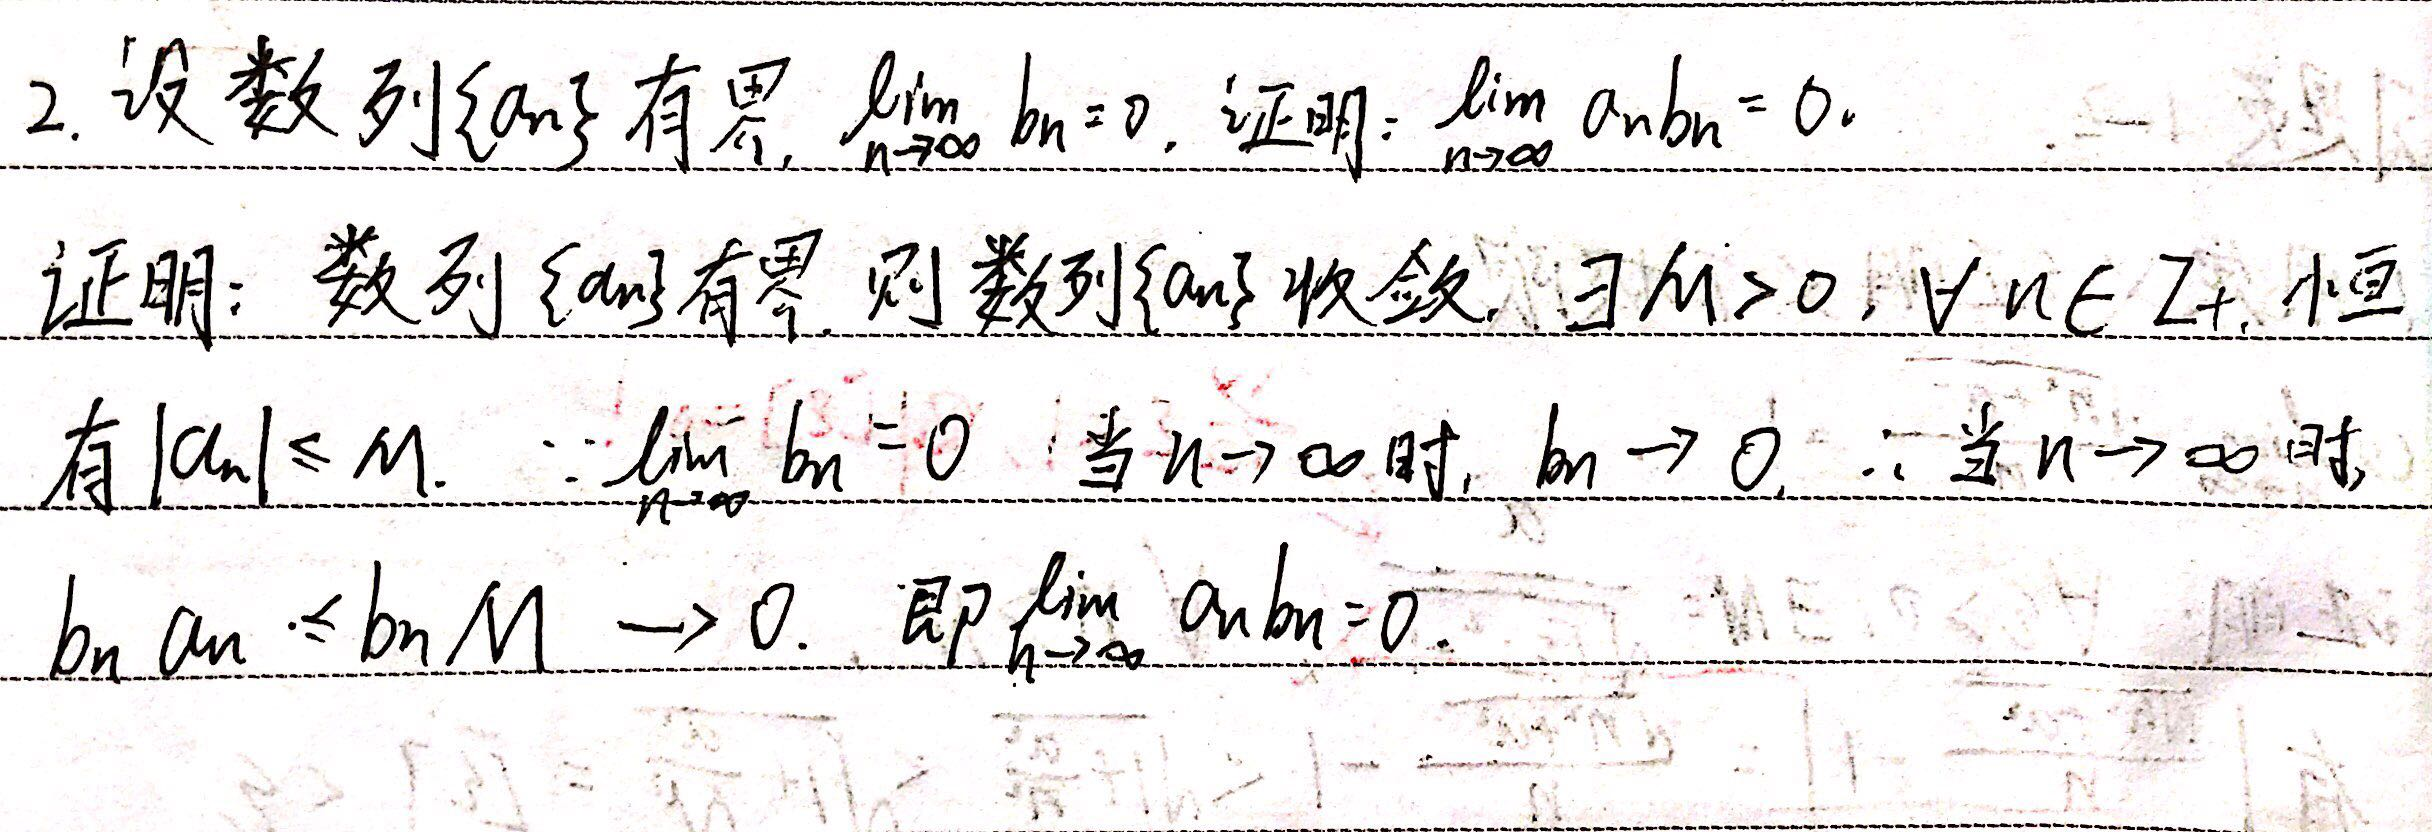
\includegraphics[width=0.9\textwidth]{./images/ch01/HWR/anbn0-2.jpeg}
\end{frame}

\begin{frame}{哪里不太对?}
	\centering
	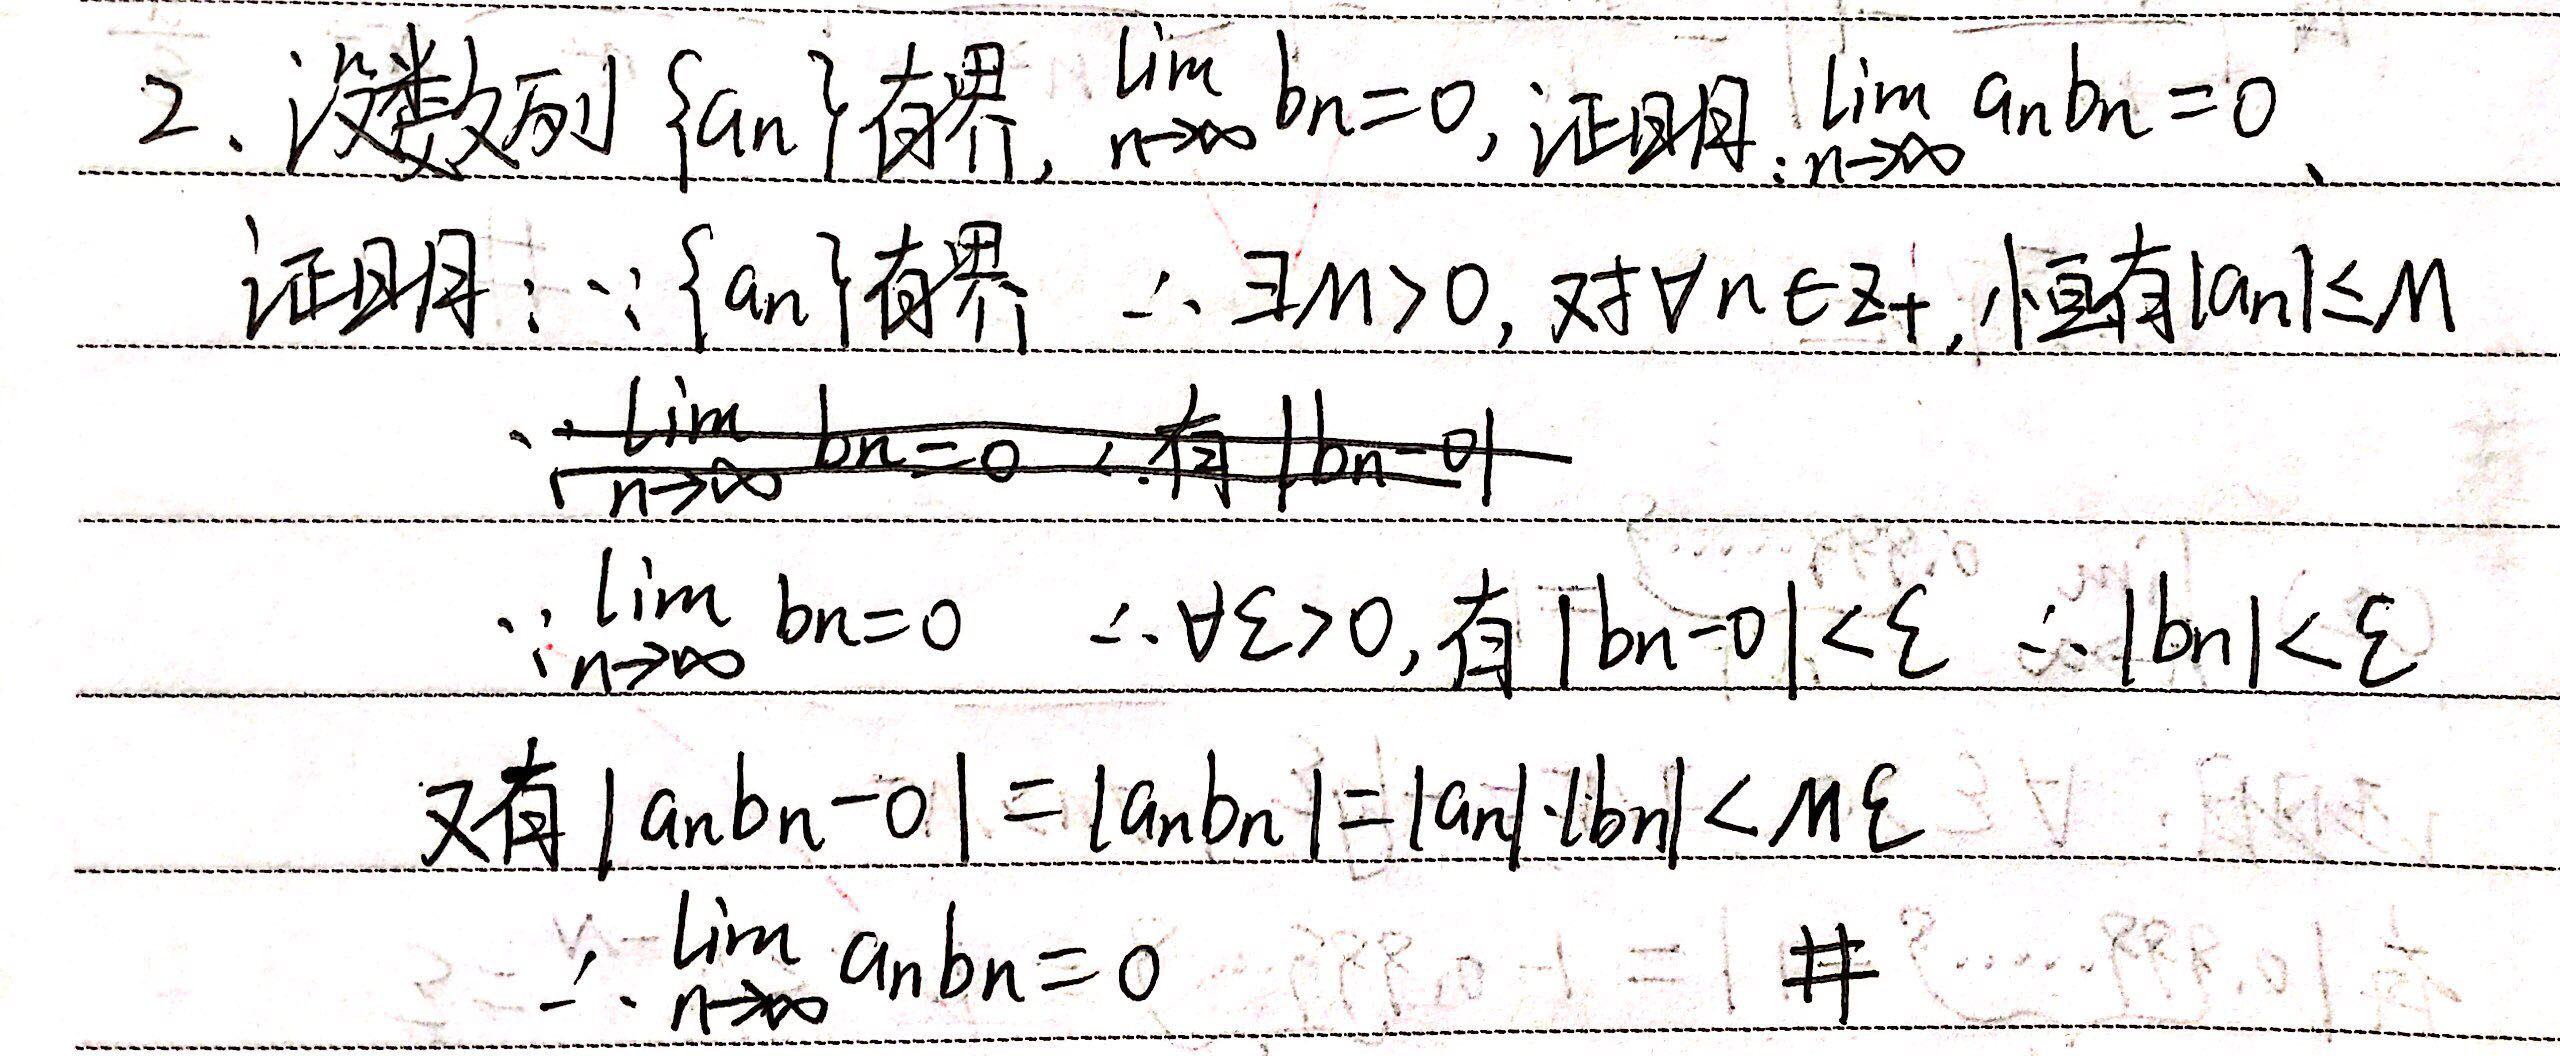
\includegraphics[width=0.9\textwidth]{./images/ch01/HWR/anbn0-3.jpeg}
\end{frame}

\begin{frame}{哪里不太对?}
	\centering
	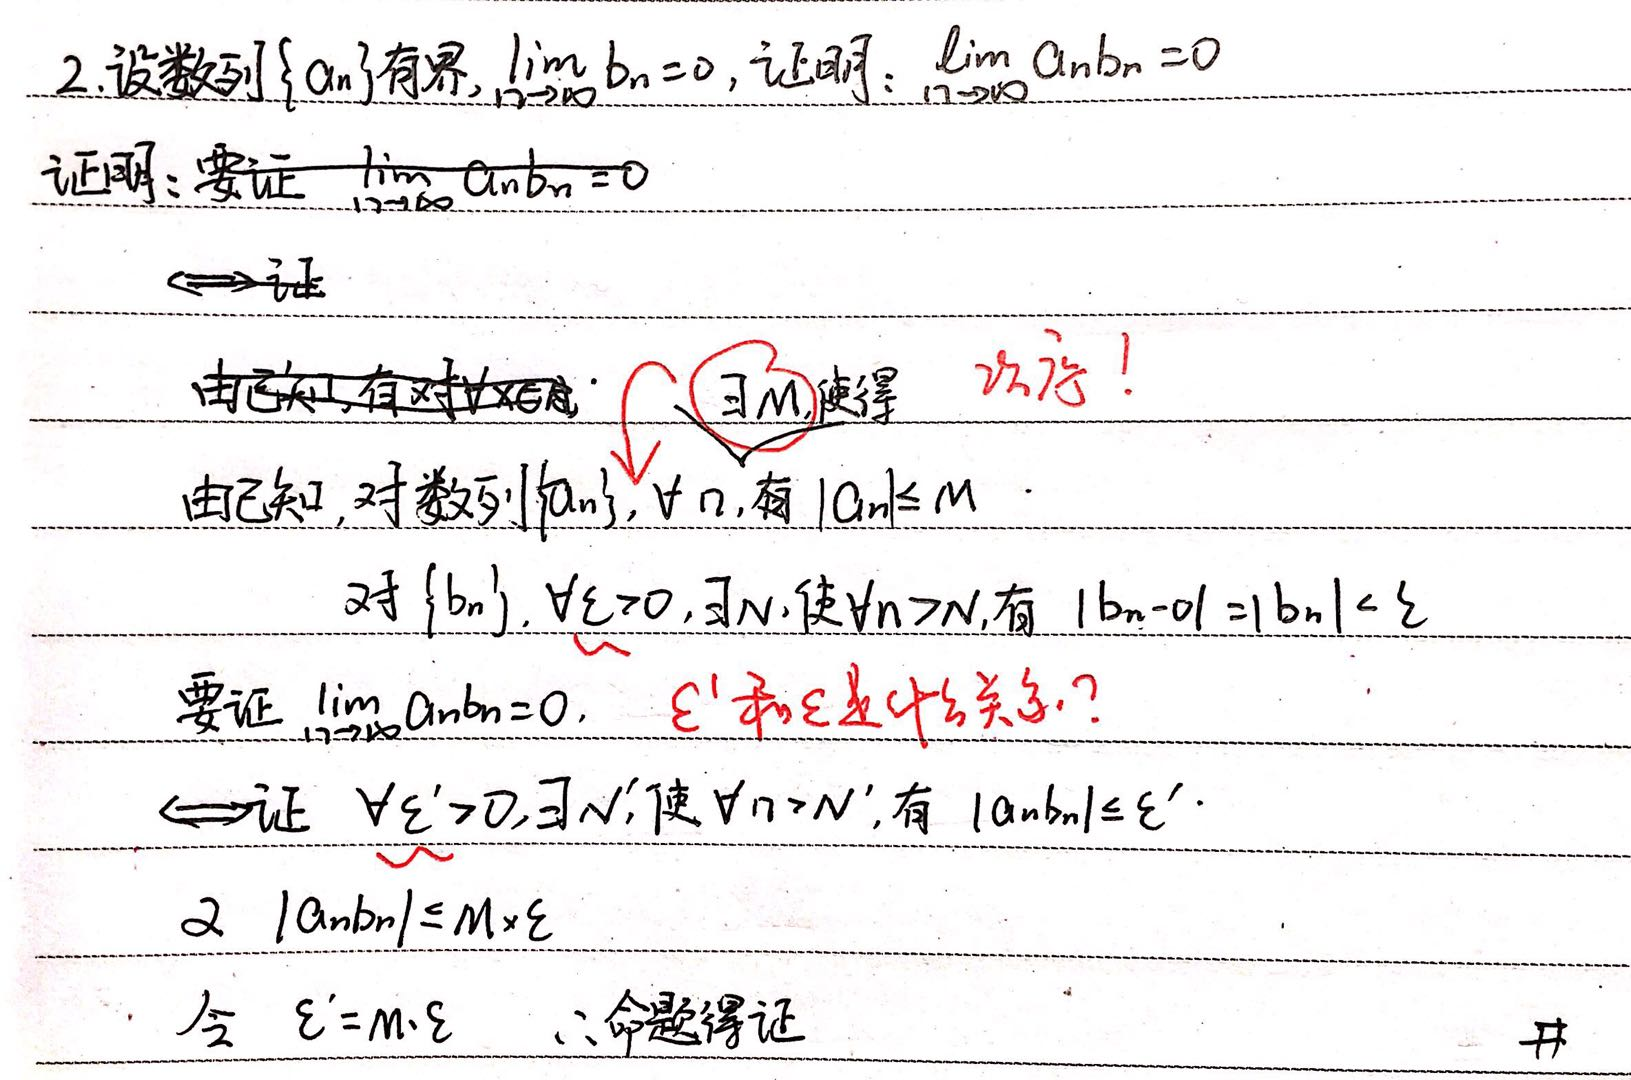
\includegraphics[width=0.9\textwidth]{./images/ch01/HWR/anbn0-4.jpeg}
\end{frame}

\begin{frame}[t]\frametitle{证明极限的性质}
\large
2.数列$\{a_n\}$有界,$\limn b_n=0$,证明:$\limn a_nb_n=0$。

证:\it 数列$\{a_n\}$有界,故存在$M>0$,对任意$n\in\mathbb{Z}_+$,均有
$$|a_n|\leq M.$$
对任意$\e>0$,令$\e_1=\df{\e}M$,由$\limn b_n=0$,存在$N$,对任意$n>N$有
$$|b_n-0|<\e_1.$$
综上,当$n>N$时,总有
$$|a_nb_n-0|\leq M\e_1=\e,$$
由数列极限的定义,即证。\fin
\end{frame}

\begin{frame}[t]\frametitle{证明极限的保号性}
\large
3.设$\limn a_n=a\ne 0$,证明:存在$N\in\mathbb{Z}^+$,对任意
$n>N$,有$|a_n|>|a|/2$。

证:\it 对$\e=\df{|a|}2$,由$\limn a_n=a$,存在$N\in\mathbb{Z}^+$,
对任意$n>N$,有
$$|a_n-a|<\e=\df{|a|}2.$$
由绝对值不等式$|a_n-a|>||a_n|-|a||$,故
$$||a_n|-|a||<\df{|a|}2.$$
也即
$$-\df{|a|}2<|a_n|-|a|<\df{|a|}2,$$
由其中的右侧不等式可知$|a_n|>\df{|a|}2$,即证。\fin
\end{frame}

\begin{frame}
	\centering
	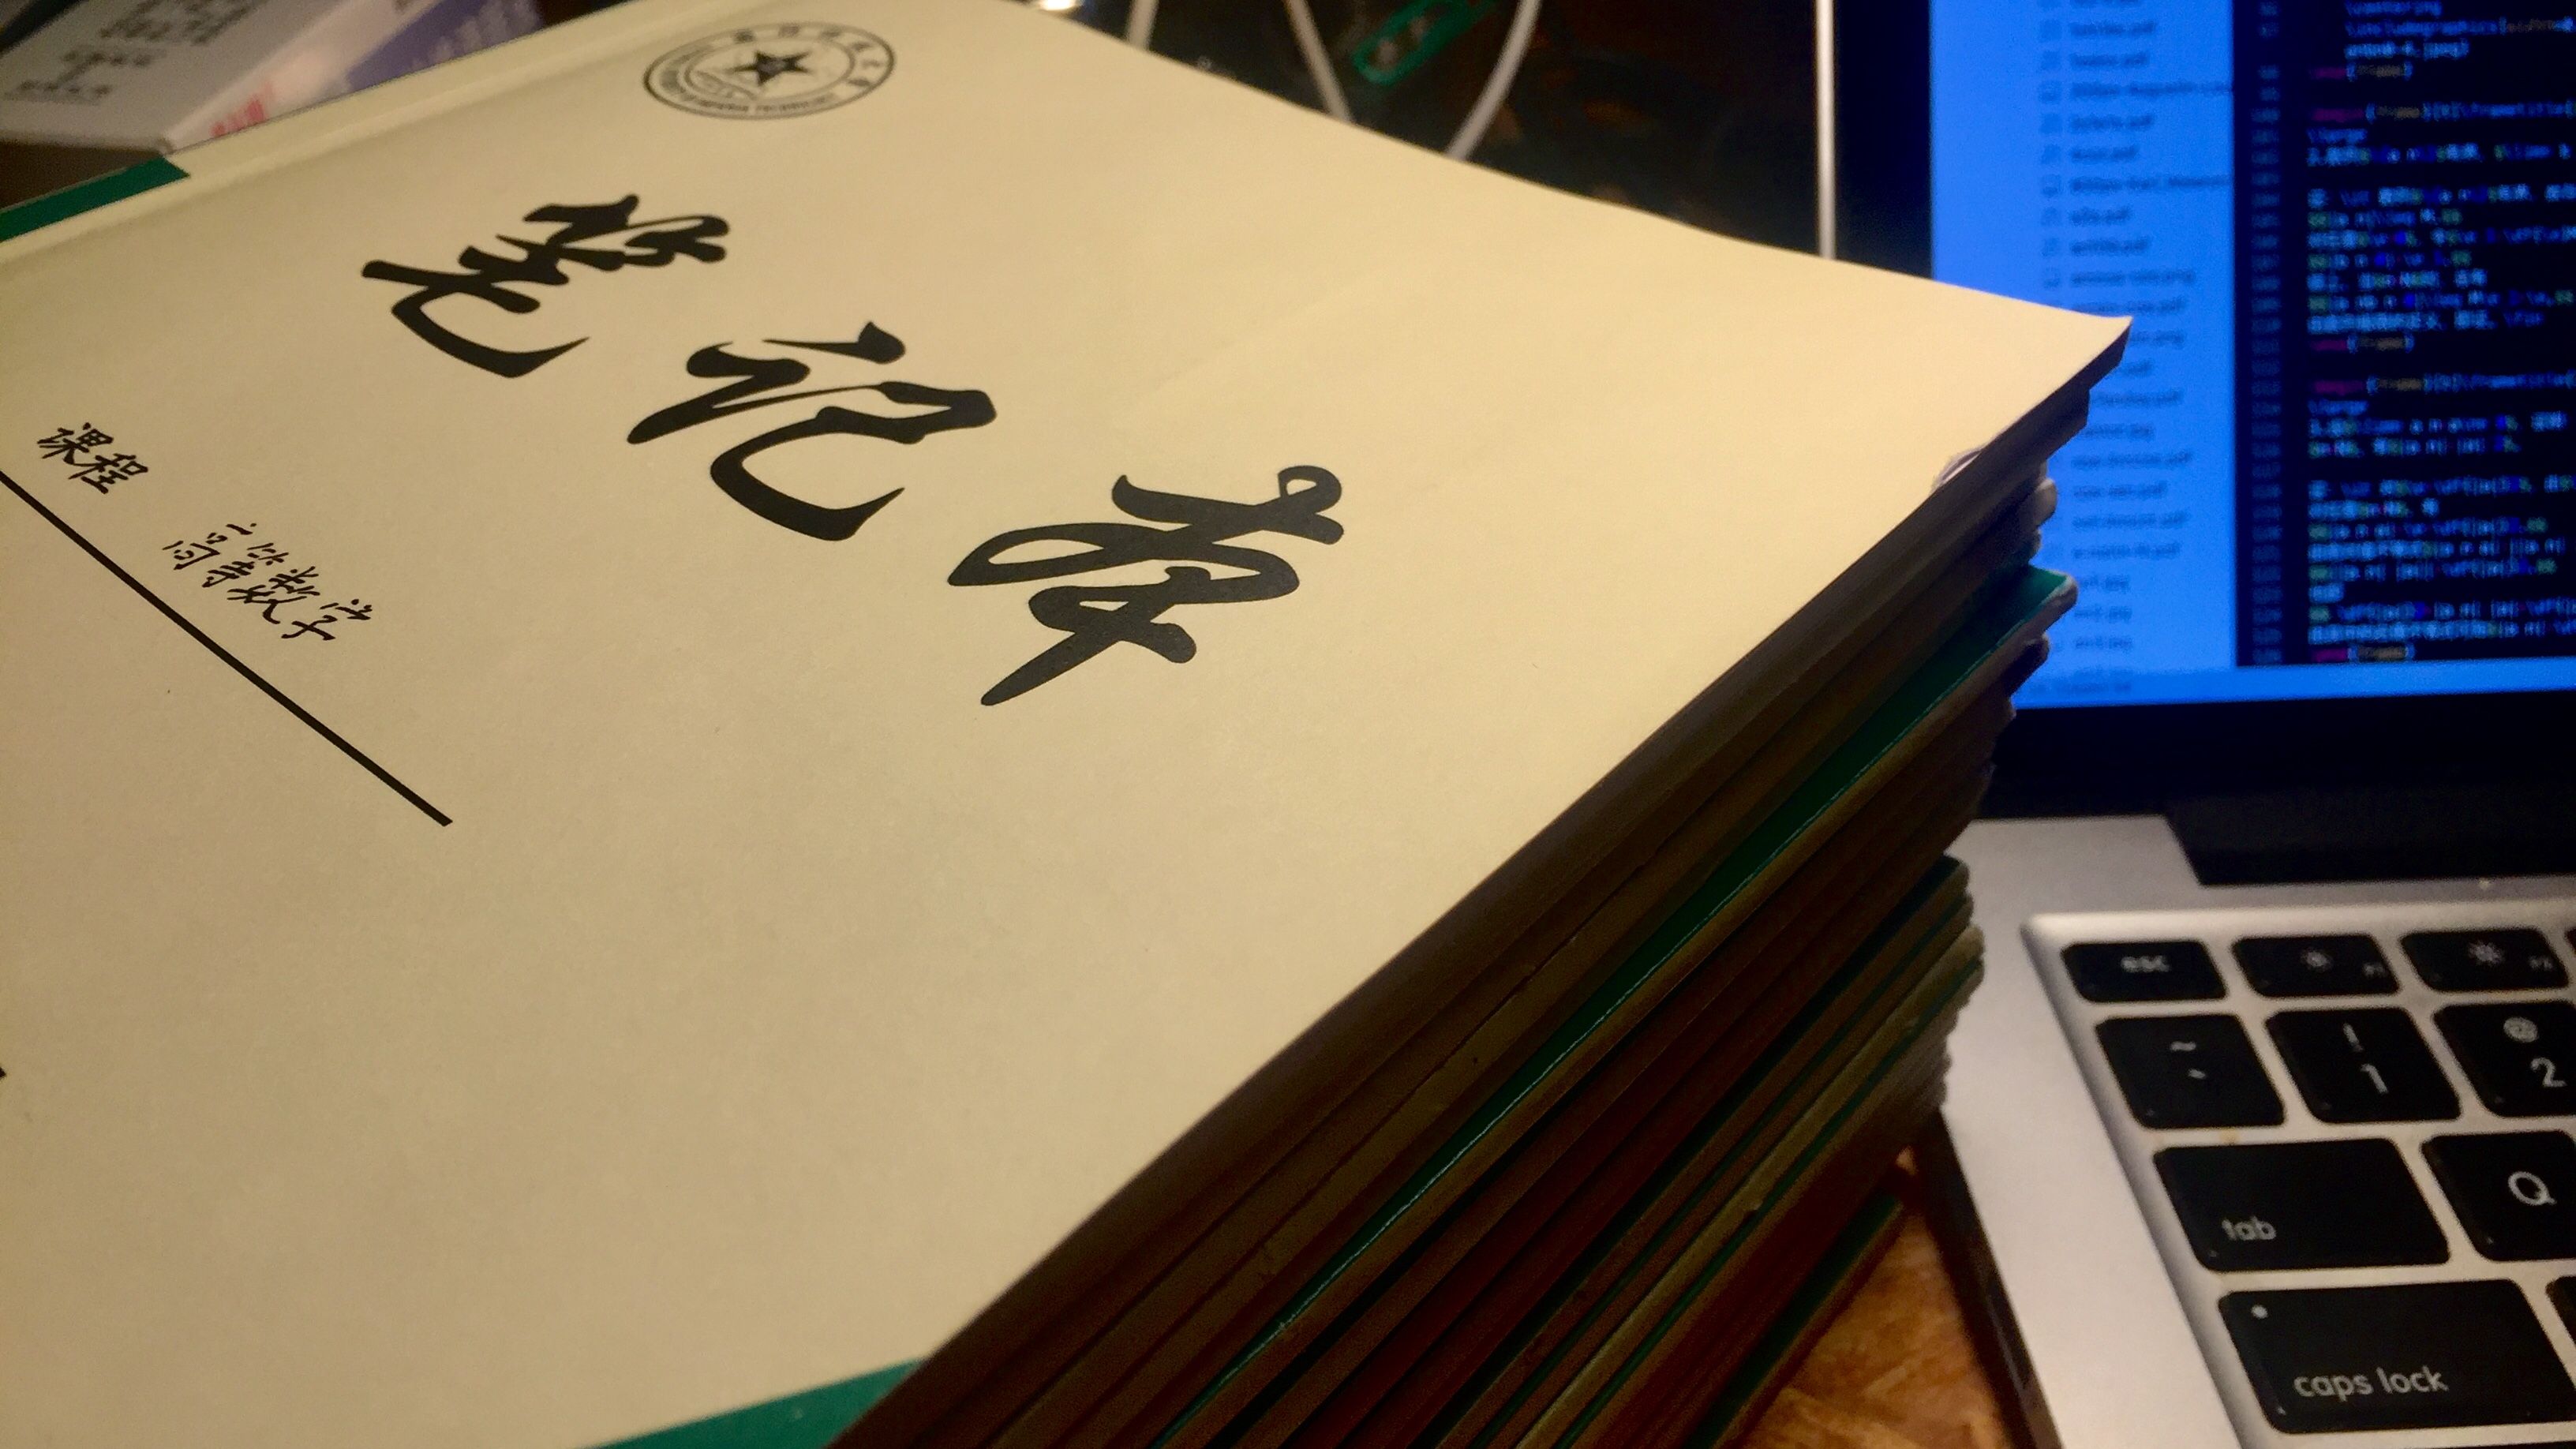
\includegraphics[width=0.9\textwidth]{./images/ch01/HWR/notebook.jpg}
\end{frame}